\documentclass{article}

\usepackage{graphicx}
\usepackage{float}

\graphicspath{{img/}}

\begin{document}

\title{Project Deliverable 5}
\author{Group 5}
\date{}
\maketitle

\section{Pathfinding Progress}

The A* implementation has been made, and using it, a testing framework. A* 
accepts a map in the form of an $x$ domain and $y$ range to define the bounds
and a list (HashSet) of obstacle locations and returns a path as the set of
significant points. The agent will, according to its current knowledge of the
grid, be able to travel directly between any two points in order. Think of them
as the turning points in the path. The accuracy of this path was tested for
many types of graphs, to be explained later.

In order to keep as much of the testing consistent, D* Lite implementation
began as a direct copy of A*. Building off of this starting point rather than
implementing the algorithm from scratch allows for individual programming
decisions to play a minimal in the result of the overall program. Though
the D* Lite program is not fully functional according to its documentation,
it logs all of the same events as A*.

\section{Map Progress}

The original A* program was run and tested using maps provided by MIT's
BattleCode. Due to its flexible structure, it was easily adapted to our
own map generator. Thanks to a complete accident regarding a still-unknown
bug in the implementation of a maze-generating algorithm, we have stumbled
upon what Alex calls ``WTF Grid'', a very realistic-looking map generator.
Figure 1 demonstrates this.

\section{Framework}

A lightweight testing framework was also implemented. This framework allows
the programs to log their choice of events as they run. Node comparisons,
path insertions, and heuristic calculations are to name a few. The actual
events logged are completely determined by programs importing it, and this
testing framework could theoretically be exported to its own library to be
used for other projects. The output is currently a comma separated value
file, but a conversion to JSON format is likely.

\section{Moving Forward}

Obviously, D* Lite needs to be implemented. Then, the following tests need
to be run to compare the algorithms:

\begin{itemize}
    \item Timing and number of each type of instruction
    \item Grid size on the efficiency
    \item Changing potentially unrelated information after pathplanning is run
    \item Changing vital information after pathplanning is run
\end{itemize}

Due to the format of the save file, generating a visual representation of all
of these tests will be near-trivial. Collecting all of this into a video
and discussing D* Lite in a presentation comes last. Admittedly, all that has
been planned so far for the video is that this day will have to be reported,
but explaining the brief history, reasons it is convenient, and how it works
are on the list of potential topics to be covered.

\section*{Appendix}

\begin{figure}[H]
    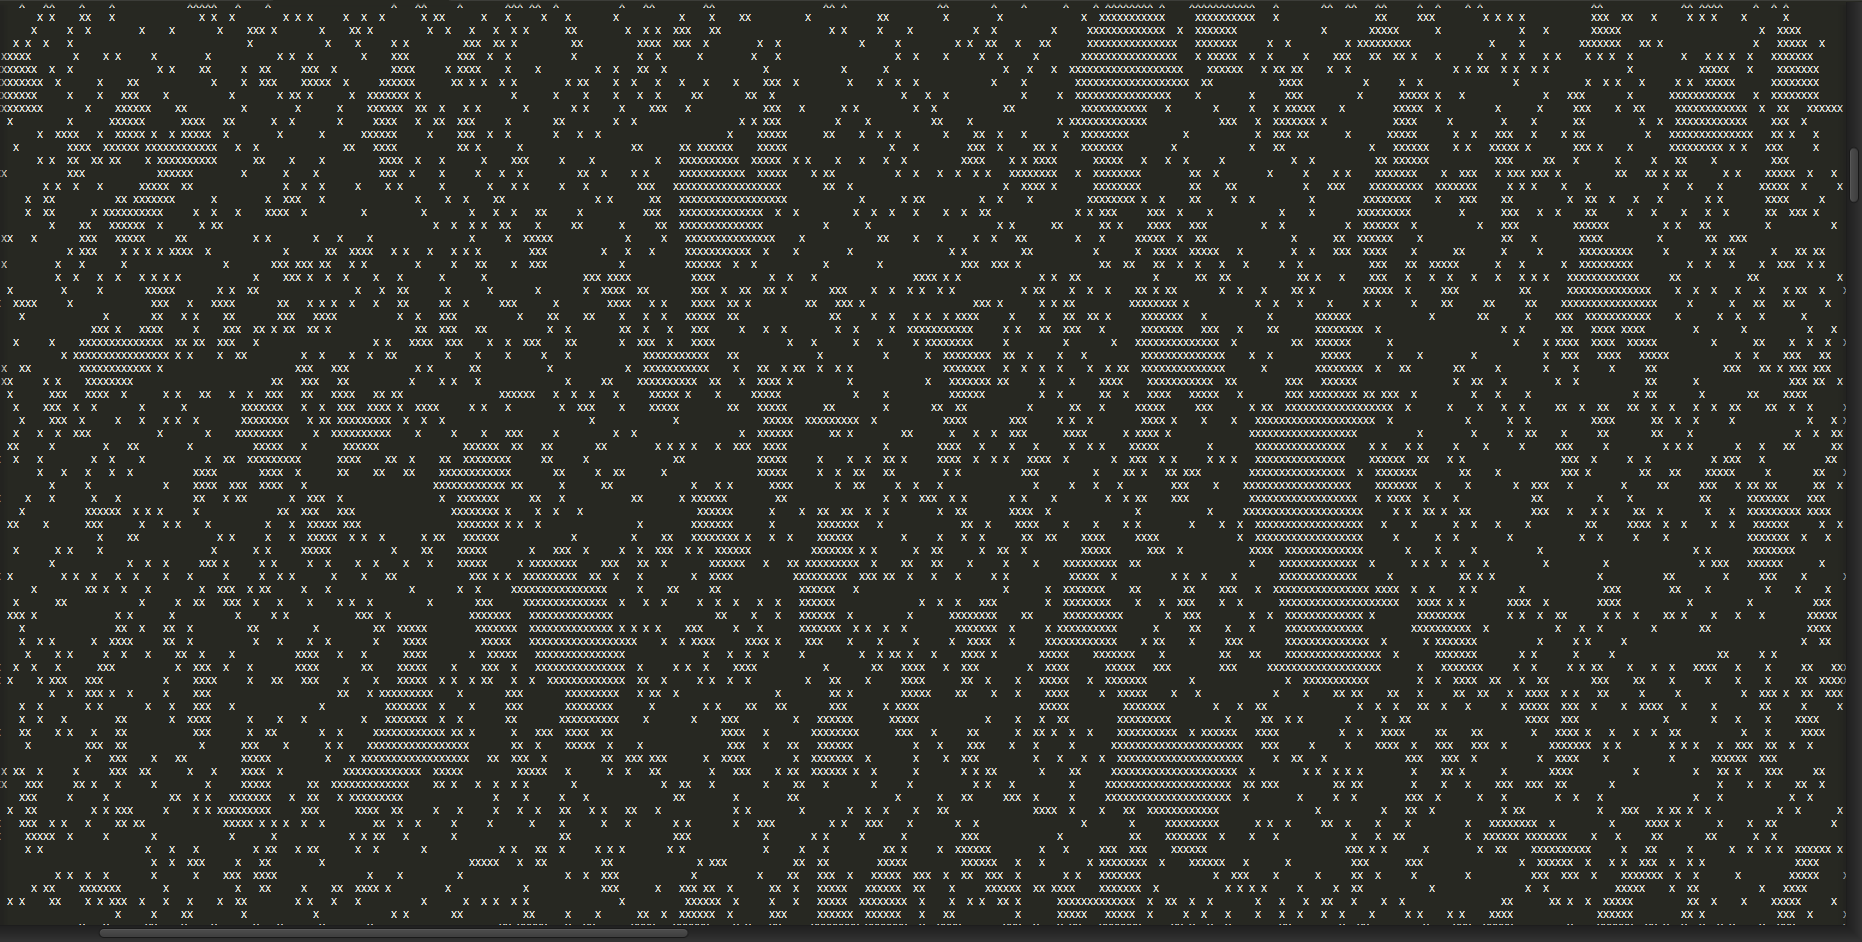
\includegraphics[scale=0.2]{map}
    \caption{A small fraction sample output generated by WTF Grid}
\end{figure}

\end{document}